\section{Research Background}
Biometrics technology is a technology that identifies or verifies individuals based on their physiological characteristics such as fingerprints, face, iris, etc. or behavioral characteristics such as voiceprints and handwritten signatures. This technology is widely used in security authentication, financial transactions, access control systems and other security areas [1] for personal identification or verification. In the identification scenario, the system will identify the user profile already in the system database based on the physiological or behavioral characteristics provided by the user. This scenario is applicable to fingerprint, iris identification of personal identity, etc. Secondly, in the verification scenario, the user needs to provide the system with verified identity and characteristic information, and the system will judge whether the current user is the declared user based on the stored characteristic information and the information currently provided by the user, which is applicable to the scenarios of declaring personal identity and providing personal characteristic information, such as the unlocking of smart phones and international border crossing.

Handwritten signature is a more important individual behavioral characteristic in daily life, and as the main characteristic for verifying personal identity in legal, financial, administrative and other fields, because it cannot be intruded during the collection process, handwritten signature is also regarded as one of the main characteristics of many technologies for verifying personal identity. Handwritten signatures produce different writing styles, such as regular and cursive, depending on the individual's writing habits. Even with the passage of time, the personal writing style may change, and the signature (defined as Query) provided by the user after a certain period of time may differ from the reference signature (defined as Reference) previously entered into the system. As a result, there will be some difficulties in comparing the verification of the user's handwritten signature, for example, there will be differences in the angle of the bending strokes, the length of the straight line, and the hook at the end of each character on the personal signature. As mentioned above, the handwritten signatures may be slightly different in the end depending on individual writing habits. Therefore, in order to obtain a user's identity privileges, some people may maliciously forge handwritten signatures to pass the security and privacy checking system, or even practice for a long time in order to achieve handwritten signatures of similar styles as a certain user. As a result, academics have launched a series of studies on handwritten signature verification, hoping to design a relevant model to help relevant staff to more efficiently complete the process of more repetitive handwritten signature verification work, so that more staff to participate in the more core work.

In academia, handwritten signature verification is categorized into two types, offline and online, depending on the data collection route. The collection process of offline handwritten signatures is obtained after the user's writing process on paper; online handwritten signatures are collected by using a digitizing station, and the collected handwritten signature images may be affected by the equipment, such as the position of the pen, tilt, and pressure, etc. [3]. In addition to the different data collection routes are categorized into different types of handwritten signature verification, scholars have defined two types of branching tasks, Writer-Independent (WI) and Writer-Dependent (WD) to evaluate the model algorithms.The WI task refers to the modeling structure where a handwritten signature image is inputted, and the handwritten signature is verified based on the referencesignature and the The WI task refers to the input of a handwritten signature image into the model structure, and based on the features extracted from the reference signature and query signature, it determines whether the query signature is forged or not, while the WD task adds the author id to the input of the WI task, and based on the author id, it uses the corresponding author classifier to determine whether the query signature is forged or not. These two branching tasks, although both output the label category of query signatures (genuine or forged) at the end, can reflect the different performance of the model to different degrees. The WI task focuses on learning the global characteristics of the signature population, does not need to learn a separate author classifier for each user, and has the excellent extensibility of not requiring re-training for new users, and at the same time can reflect the generalization and discriminative ability of the model. The WI task focuses on learning the global features of the signature group, does not need to learn an author classifier for each user individually, has excellent scalability without re-training for new users, and can reflect the model's generalization and discriminative ability; the WD task additionally trains an author classifier for each user individually, which can take into account the high accuracy of different styles of signatures of individual authors that are still considered to be real signatures, but needs to collect a sufficiently large number of samples for each user, with a high cost of training and a weak generalization ability. Thus the WI and WD tasks can reflect the overall performance of the model to different degrees, and the model performance is comprehensively evaluated according to the evaluation indexes of the two tasks.

With the development of the level of technology, the field of artificial intelligence has been able to generate fake pictures based on the sample images and keywords provided by the user, and it is difficult for normal people to identify the real and fake with the naked eye. Therefore, there will be part of the artificial generation of forged signature behavior, so as to achieve the fake to pass the verification of the security system, resulting in personal privacy, property invasion, theft and other dangerous consequences. Relying on manual power to verify will have certain social risks and judgment errors, so the study of offline handwritten signature verification, to a certain extent, can reduce the risk of forged signatures through the verification of the relevant algorithmic models to help minimize the error of manual verification, so as to better ensure personal privacy and property security.

\section{Research Motivation and Importance}

This paper focuses on the offline handwritten signature verification task, which is essentially a derivative branch of the image classification task. Unlike the traditional image classification task, the offline handwritten signature verification task requires the input of a pair of signature image samples from the REFERENCE and QUERY pairs, and the WD task requires an additional input of an author id to train an author-independent classifier. The offline handwritten signature verification model will extract relevant image features based on the input reference and query signature images, and compare the features to output genuine or forged category labels. Thus the task is challenging and innovative, the design of the model or algorithm architecture not only needs to consider the criticality of the model to extract a pair of image features, the model architecture of the isotropic dual-stream will directly affect the criticality of the features extracted from the referencesignature and query-signature images, and once the extracted features don't have so important information, it will lead to a drastic decrease in the model's ability to make judgments. At the same time, due to the definition of the WI and WD tasks and the real-life application scenarios, it is required to have a high accuracy rate and generalization ability to prevent personal privacy and property infringement, but also to enhance the demand for the performance of the model, which makes the design and experimentation of the offline handwritten signature verification model a very challenging image task.

In the design of offline handwritten signature verification model, it is divided into two parts: feature extractor and author classifier for WD task. In the past research of scholars, most of the data cluster features based on sample distribution and other data cluster features to manually design the image feature extraction method, to take the traditional machine learning approach to determine whether the signature is forged or not [1], such as taking the distance between the features or SVM to determine whether the signature is forged or not. But this manually designed features have the defects of specific data clusters, it must require the data set of the author's signature style uniformity, subtle differences will be as outliers leading to the traditional machine learning methods to determine the accuracy of the decline in the accuracy of the work, but the actual production work is required to have these certain differences in the tolerance of the degree of the work, so this method of extracting the features to take the artificial design is gradually phased out. Scholars hope to have an image feature extractor that focuses more on a certain part of the image and does not need to intervene many times. With the rapid development of deep learning in the past six years, convolutional neural network (CNN) with shared parameters for local field of view operations has achieved good results in traditional image classification tasks such as MNIST, ImageNet, and compared with the traditional machine learning methods, the accuracy and generalization ability of CNN is even better than that of traditional machine learning methods. The accuracy and generalization ability of CNNs have been further verified in comparison with traditional machine learning methods. As a result, scholars in the field of handwritten signature verification have introduced CNN as a feature extractor, and experiments have proved that the accuracy and generalization ability of this approach has made a great breakthrough compared with previous methods [2].

Even though CNN's ability to extract image features is outstanding, its core idea of convolutional kernel operation has a certain local field of view reinforcement learning ability, which can focus on the local features of the image; however, for handwritten signatures not only need to pay attention to the degree of the corners of the font strokes, but also need to pay attention to the overall style of the signature image, fonts, and other factors, which may result in the case of the signature of the same author in a different location, so CNN as a feature extractor still has some defects. With the development of the field of natural language processing, the appearance of Transformer [9] with global feature learning attracted the attention of scholars, and then scholars in the field of image introduced the Encoder-Decoder architecture of Transformer for experiments on classification tasks [?]. The experiments proved that this approach outperforms CNN's feature extractor in the case of model parameter convergence, but the training conditions to reach model parameter convergence are more demanding because Transformer's attention mechanism needs to learn the whole image, whereas CNN adopts the way of sharing parameters to learn the local features of the image, so that the model convergence can be reached more quickly, but in the practical use, the generalization ability is poor. However, in practice, the generalization ability is poor, and the dataset needs to be constantly fine-tuned to achieve higher model performance. As a result, CNN is derived as Backbone to extract multi-channel feature maps, which are flattened as feature vectors and entered into the Transformer to perform global attention feature operations [?] In order to achieve the multi-channel feature map in the absence of overall information, after the Transformer's attention mechanism to strengthen the characteristics of the overall information, experiments have proved that this way can be more effective in learning image features, models and thus achieve better accuracy and generalization ability. In summary, the CNN+Transformer style model architecture has become a mainstream framework in the image field in recent years, and it has also been introduced in offline handwritten signature verification tasks, and experiments have proved that this style of model architecture has a good model performance[?] Therefore, the offline handwritten signature verification model based on Transformer proposed in this paper is also a CNN+Transformer style model architecture, which conforms to the development trend of this field in deep learning in recent years, and adds multi-scale fusion features based on it, so that it can learn the signature image at multiple scales while meeting the increasing requirements of high-definition image resolution. The features such as font stroke corners make up for the shortcomings of multi-channel feature maps in terms of scale after CNN. In the final output classification stage, unlike the traditional image classification task, the model proposed in this paper will collect the features from previous modules in the final output, and perform overall stitching for category label prediction or model training, which has been proven to be effective [?]. . The challenge of this research is how to effectively use multi-scale fusion features for category prediction and model training. This way of training and prediction using the overall model features can better train the model weights of each part of the model as a whole, and the model training to the convergence stage will surpass most of the previous deep learning model architectures, and it provides a novel idea for the related fields to integrate the feature approach of convolutional neural networks and attention mechanisms. For related fields, it provides a novel idea to integrate the features of convolutional neural network and attention mechanism, which provides a certain design idea for the subsequent more concise fusion module; on the contrary, this approach will increase the computational reasoning pressure of the equipment and the cost of model training, which needs to be proved to be effective through a variety of experiments.


\section{Research Objects}

The OSVTF architecture proposed in this paper, as a whole, is a model designed based on the idea of twin networks, as shown in Fig. 1.

\begin{figure}[htbp]
    \begin{center}
        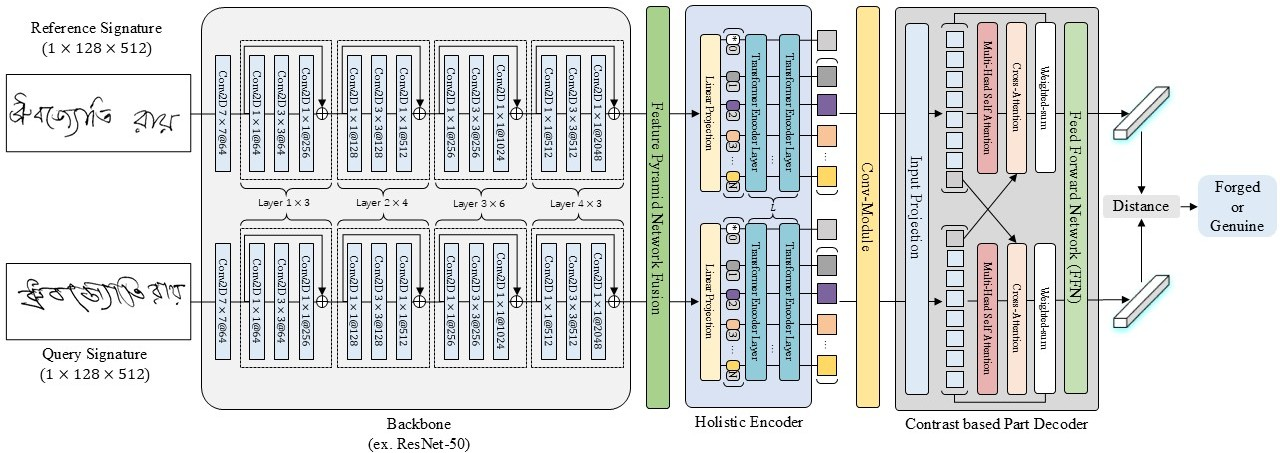
\includegraphics[scale=0.6]{figure/OSVTF.jpg}
    \end{center}
    \caption{OSVTF Structure}
    \label{fig:OSVTF}
\end{figure}

The core idea of a twin network is two sub-networks with shared weights that accept two inputs and output two feature vectors, and subsequently use a distance function to compute the similarity [?] . In the WI and WD tasks of offline handwritten signature verification, a pair of images of the inputreference and query signatures are input, so the overall architectural aspect is referenced from TransOSV [?]. On the basis of TransOSV, backbone and FPN Fusion modules are added, and a series of optimizations and adjustments are made to Encoder, Conv-Module and Decoder, which are more conducive to the change and learning of the features of each part, and the experimental part needs to confirm that these modules can improve the model's ability to judge forged signatures and generalize the model to different scenarios. Experimentation
In the overall research plan and experiments, the two general directions of WI and WD are still adopted to evaluate the model performance and quality, based on which the multi-channel feature map of CNN and the attention mechanism of Transformer will be visualized, and it is necessary to pay attention to whether these modules are able to better grasp the important feature information of the image in the learning of image features. In addition, there are various ways of fusion of multi-scale features, such as Mask-RCNN [?]. The Feature Pyramid Network Style (FPN-Style) [?] is adopted. , this fusion approach includes but is not limited to mean accumulation, direct summation, and splicing, so these fusion approaches will be followed by model training with control variables to obtain the best performance fused multi-scale feature map approach. In addition, the previous twin network approach is based on the distance function to calculate the similarity to complete the related tasks, whether this approach can still be effective after the addition of multi-scale fusion of features needs to be verified to some extent, this paper will refer to the traditional image classification task of the classification of CNN processing, the addition of a global average pooling layer as a classifier to classify the features of the classification label prediction, so as to determine whether it will be better than the previous distance similarity judgment.
In summary, this paper will be divided into three parts of the research phase: 1. Initially, the OSVTF model architecture will be trained in the model cycle to verify whether the optimization and adjustment scheme of the multi-scale features and model can be improved on the original architecture; 2. For the multi-scale fusion method of the FPN Fusion module, a small fine-tuning training will be taken on the basis of the first phase by adopting the control variable method for the model, and the optimal multi-scale feature fusion method will be screened out. The best multi-scale feature fusion method; 3. For the WI task, a global average pooling classifier is added in the final classifier stage, which is compared with the previous method of distance similarity prediction for offline handwritten signature verification, so as to judge the advantages and disadvantages of the two classifiers, and a better classifier is adopted for experiments in the WD task to verify whether it works.



% 緒論的主要作用是:要告訴讀者本文的研究主題、論證本研究主題的價值所在、提出作者對研究問題的主觀答案。通俗地講就是:研究動機、問題背景,選題原因和實際工作的關係、研究的重要性、研究目的、研究假設或待解決問題、名詞及定義以及研究範圍和限制等。

% 文獻綜述:是描述目前的研究現狀並作簡要分析。可以反映作者研究的功力和閱讀文獻的數量,是否找到研究問題的關鍵文獻及抓準文獻的重點。評述是否切中要害,是否有獨到見解。忌諱採用講義式將有關研究課題的理論和學派簡要地陳述一篇;忌諱輕率批評前人的不足和錯誤;忌諱含糊不清,採用的觀點和內容不清楚來源。











% The main function of the introduction is to put forward the research topic of this paper, demonstrate the value of this research topic and put forward the author's subjective answer to the research questions \cite{wang2019}.

% As far as the authors know, no much attention is paid to the development of computationally efficient methods for siphons in a Petri net.

% \section{Cite in the text}
% 註意:作者人數不同,在參考文獻在文中的引用格式也不同!

% Fang develops a method for supervisor synthesis ... \cite{zhang2019}.

% A plethora of computationally efficient methods are reported in \cite{zhang2019, wang2019}, which are polynomial with respect to the size of a plant and the number of fault types. However, the diagnosis strategy in \cite{wang2019} behaves more competitively if the number of controllable events is far more less than that of the uncontrollable events. 

% Wang and Li develop a method for supervisor synthesis ... \cite{wang2019}.

% Zhao {\it et al.} develop a method for supervisor synthesis ... \cite{zhaoliu2019}. (Three or more authors)

% \section{Format of references}

% 1. 不要引用難於找到的文獻,如在英文論文中引用中文論文。

% 2. 不要遺漏重要和必要的文獻,以免評閱人對研究者的水平產生質疑。

% 3. 參考文獻的順序按作者姓的字母升序排列,同樣作者的年代前的在前。

% 註意: 關於期刊、會議、專著-書,博士論文和專利報告等等,都有不壹樣的格式。在引用時,應該多加留意!


% E-books:

% [1] L. Bass, P. Clements, and R. Kazman, {\em Software Architecture
% in Practice, 2nd ed. Reading, MA: Addison Wesley}, 2003.
% [E-book] Available: Safari e-book.

% Single Author:

% [1] W. K. Chen, {\em Linear Networks and Systems}. Belmont, CA:
% Wadsworth Press, 2003.

% Edited Book:

% [2] J. L. Spudich and B. H. Satir, Eds., {\em Sensory Receptors and
% Signal Transduction}. New York: Wiley-Liss, 2001.

% Selection in an Edited Book:

% [3] E. D. Lipson and B. D. Horwitz, ``Photosensory reception and
% transduction,'' in {\em Receptors and Signal Transduction}, J. L.
% Spudich and B. H. Satir, Eds. New York: Wiley-Liss, 2001, pp.
% 1–64.

% Three or More Authors:

% [4] R. Hayes, G. Pisano, and S. Wheelwright, {\em Operations,
% Strategy, and Technical Knowledge}. Hoboken, NJ: Wiley, 2007.


% Manual:

% [5] Bell Telephone Laboratories Technical Staff, {\em Transmission
% System for Communication}, Bell Telephone Lab, 2005.

% Application Note:

% [7] Hewlett-Packard, Appl. Note 935, pp.25–29.

% Technical Report:

% [8] K. E. Elliott and C. M. Greene, ``A local adaptive protocol,''
% Argonne National Laboratory, Argonne, France, Tech. Report.
% 916-1010-BB, 7 Apr. 2007.

% Patent/Standard:

% [9] K. Kimura and A. Lipeles, ``Fuzzy controller component,'' U.
% S. Patent 14, 860,040,14 Dec., 2006.

% Paper Published in Conference Proceedings:

% [12] J. Smith, R. Jones, and K. Trello, ``Adaptive filtering in data
% communications with self improved error reference,'' in {\em Proc.
% 16th IEEE International Conference on Wireless
% Communications}, Taipa, Macau SAR, China, 2004, pp. 65–68.

% Papers Presented at Conferences (unpublished):

% [13] H. A. Nimr, ``Defuzzification of the outputs of fuzzy
% controllers,'' presented at {\em 5th International Conference on
% Fuzzy Systems}, Cairo, Egypt, 2006.

% Thesis or Dissertation (unpublished):

% [14] H. Zhang, ``Delay-insensitive networks,'' M. S. thesis,
% University of Chicago, Chicago, IL, 2007.

% Article in Journal:

% [15] K. A. Nelson, R. J. Davis, D. R. Lutz, and W. Smith,
% ``Optical generation of tunable ultrasonic waves,'' {\em Journal of
% Applied Physics}, vol. 53, no. 2, pp. 1144–1149, Feb. 2002.

